\chapter{Methods}\label{methods}

For this project, I am interested in two factors that help characterise the cancer mutation profile: genomic location effect (GLE) and sequence context effect (SCE; Figure \ref{fig:workflow}). I investigated each factor on two complementary scales: statistical analysis of whole disease and cancer classification for individuals. The former somewhat plays the role of a biological basis for the latter, whereas the latter could validate the patterns detected by the former.

\begin{figure}[h!]
    \centering
    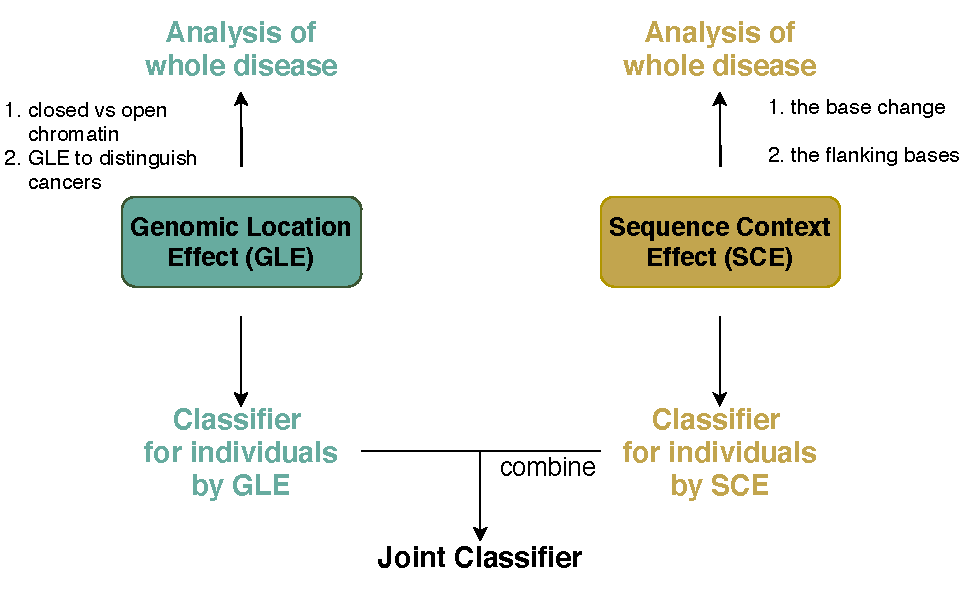
\includegraphics[scale=0.85]{graphics/workflow.pdf}
\caption{}
    % \caption{\textbf{Project workflow for understanding cancer mutagenesis data and exploiting it for cancer classification.} On one hand, cancers were analysed on the whole disease scale, which considered mutations from all donors of the same diseases as a whole. This magnified the signals in the data and made it easier for understanding the mutagenesis process. On the other hand, the information from the factors analysed above was used for training a classifier on the individual donor scale, meaning that this classifier could potentially be applied to a new patient's mutation data to predict their cancer. This followed a standard machine learning training procedure, outlined in Section \ref{methods:ml}.}
    \label{fig:workflow}
\end{figure}


\section{Data description}
\subsection{PCAWG - Mutation data:} 
The critical source of data for the project is the Pan-Cancer Analysis of Whole Genome (PCAWG) project \citep{Campbell2020}. This data consists of whole genome sequencing of both cancerous and healthy tissues (mostly blood) for all cancer patients. PCAWG relies on contrasting the cancerous against healthy tissues to determine whether a mutation is a \gls{sommut}. Identifying mutations by combining three established pipelines (Sanger \citep{Jones2016CgpCaVEManWrapper:Data}, EMBL/DKFZ \citep{Rimmer2014IntegratingApplications}, and Broad \citep{Cibulskis2013SensitiveSamples}), the project provides a valuable resource, which covers 2658 cancer samples from 28 cancer types, for studying cancer mutagenesis.

This project is limited to somatic \glspl{point_mut}. I sampled 12 cancers whose DHS data for the putative original cells is also available. A summary of the mutations for the 12 cancers can be found in the appendix Table \ref{tab:mutation_summary} and Figure \ref{fig:mutation_summary}. Mutation data for all individuals and all mutations was downloaded as a MAF file from the \href{https://dcc.icgc.org/releases/PCAWG/consensus_snv_indel}{International Cancer Genome Consortium (ICGC)}. Driver mutations were then filtered out based on \href{https://dcc.icgc.org/releases/PCAWG/driver_mutations}{the PCAWG's driver mutation project} because driver mutations are under selection pressure and have different mutation rates to passenger mutations. 

\subsection{Reference genome:} 
To reconstruct the entire cancer genome, both mutation data and a standard human reference genome are required. The human reference genome was downloaded from the \href{http://hgdownload.soe.ucsc.edu/goldenPath/hg19/chromosomes}{UCSC genome browser}. As PCAWG used Human Genome Assembly 37, the same version of genomic coordinates is used for this project. As an additional check, I also assert that the wildtype base at each mutated position and its local reference sequence context provided by PCAWG match the sequence at that position from the UCSC reference genome. 

\subsection{Chromatin status data:} 
Part of my project investigates the relationship between mutation distribution and chromatin status. Based on literature search, I identified the most likely tissue of origin for the cancer of interest, this is summarised in Table \ref{tab:encode}. DNase I hypersensitivity (DHS) data from ENCODE was downloaded for these tissues of origin from ENCODE because DHS is the canonical measure for chromatin status \citep{Thurman2012TheGenome,Klemm2019ChromatinEpigenome}. This project defines open chromatin region as the hypersensitivity range from ENCODE, and closed chromatin region as the rest of the genome.

\section{Algorithm development}
\subsection{Reproducibility} 
\href{http://git-scm.com}{Git} was used as a Version Control toll. Accordingly, the entire code history has been recorded and stored on \href{https://github.com}{GitHub}.

The entire project was done in loops, which means that most analyses were repeated on increasing scales. This not only increases the opportunity for code efficiency to be improved but also helps ensure that the algorithms are reproducible. 

While the project is too large to be shared in a thesis, all code is available upon request. 

\subsection{Developing packages}
Most core functions were written in Python \citep{van1995python}, with visualisation and some analyses written in R \citep{r}. Code was written as packages that can be installed and utilised by anyone with the permission. 

All core functions were tested under explicit hypothetical scenarios for correctness before being applied. Each of the analyses requires multiple core functions. For each analysis, core functions are combined in one command that can be run either in the command line or conventional Python platforms such as Jupyter Notebook. The \href{https://github.com/HuttleyLab/scitrack}{Scitrack} Python package was applied to these commands so that not only code, but inputs and outputs of these commands were tracked as well.

\subsection{Parallelisation}
When analysing large data sets, some steps could be considerably time-consuming, particularly the initial data filtering step and the simulation steps. Therefore, for several steps, I have written scripts that optimise code parallelisation based on the original command line. By doing this, for an analysis that executes the same processes multiple times on independent objects, these objects were ``distributed'' into different computer cores instead of being processed sequentially on one single computer. This was supported by the National Computational Infrastructure Australia.


\section{Whole disease analysis of GLE}
\section{Whole disease analysis of SCE}
\section{Training mutation-based classifier for cancers}
\subsection{Standard procedure}
\label{methods:ml}
\subsection{Combining GLE with SCE in a joint model}
